\documentclass[10pt, a4paper]{article}

% formating packages
\usepackage[a4paper, margin=1cm, bmargin=2cm]{geometry}
\usepackage{titling}
\usepackage[perpage]{footmisc}

% clickable links
\usepackage{hyperref}
\hypersetup{
	colorlinks=true,
	urlcolor=black,
	linkcolor=black
	}

% graphics packages
\usepackage{graphicx}
\usepackage{subcaption}

%math packages
\usepackage{amsmath}
\usepackage{amssymb}

\graphicspath{ {./plots/} }

% reduce title size by 1cm
\setlength{\droptitle}{-1.5cm}

% set paragraph indent to 0 and paragraph seperation to 5pt
\setlength{\parindent}{0pt}
\setlength{\parskip}{5pt}

% macros
\newcommand{\omp}{\textit{OpenMP}}
\newcommand{\simd}{\textit{SIMD}}
\newcommand{\avx}{\textit{AVX2}}
\newcommand{\mpi}{\textit{OpenMPI}}
\newcommand{\gnu}{\textit{GNU}}
\newcommand{\blas}{\textit{CBLAS}}
\newcommand{\gsl}{\textit{GSL}}
\newcommand{\C}{\textit{C}}
\newcommand{\slurm}{\textit{Slurm}}
\newcommand{\qselect}{\textit{QuickSelect}}
\newcommand{\qsort}{\textit{QuickSort}}

\begin{document}

\title{
	\textbf{Parallel \& Distributed Computer Systems}\\
	Exercise 2 -- \textit{Distributed All-KNN}
}

\author{\textit{Alexandros Athanasiadis} -- 10006}
\date{\today}

\maketitle

\begin{abstract}
	In this report I will showcase my attempt at building a program using \mpi \ in order
	to compute the All-KNN problem in a system of distributed computer nodes. I will present the
	algorithms used for the non-distributed implementation, the methods of communication between nodes 
	and the testing methods. Various figures will show the performance of the program adjusting over
	certain parameters. \\

	\noindent
	Source code at: \url{https://github.com/alex-unofficial/knn}
\end{abstract}

\section{The Problem}
The All-KNN problem is described as such: \\
given a set $S$ of $N$ input points of $d$ dimensions ($S \subseteq \mathbb{R}^{N \times d}$),
for each point $x \in S$, find the $k$-nearest points $y \in S$

To compute the Solution to All-KNN we need to solve 2 subproblems, 
\begin{enumerate}
	\item For each point $x \in S$ compute the distance to all other points $y \in S$.
	\item For each point $x \in S$ select the $k$ points with the smallest distances.
\end{enumerate}

I used the Euclidean Distance $||x - y|| = \sqrt{\sum_{i=0}^d |x_i - y_i|^2}$ 
as a distance metric, and specifically the Squared Euclidean Distance since the Square Root is 
relatively hard to compute and the distances will be sorted the same way, squared or not. 
Other distance metrics may also be used like the Hamming Distance or the Minkowski distance.

\subsection{The Squared Euclidean Distance Matrix}
The Squared Euclidean Distance Matrix (SEDM) between 2 arrays of points 
$X \in \mathbb{R}^{n \times d}, Y \in \mathbb{R}^{m \times d}$, \\
is a matrix $D \in \mathbb{R}^{n \times m}$ such that $D_{ij} = ||X_i - Y_j||$.

Implementing the SEDM can be done in 2 ways. \\

First by simply evaluating $||X_i - Y_k|| = \sum_{k = 1}^{d} (X_{ik} - Y_{jk})^2$ for all values of $i, j$. \\

Secondly by the fact that $\sum_{k = 1}^{d} (X_{ik} - Y_{jk})^2 = 
\sum_{k = 1}^{d} (X_{ik}^2 - 2 X_{ik} Y_{jk} + Y_{jk}^2)$ we can construct the arrays $X^2$ and $Y^2$ 
such that each row of these arrays shall contain the product $X_i^2$ and  $Y_j^2$, and use a highly efficient
linear algebra library like \blas \ to compute $X \cdot Y^T$. Then by iterating over $i$ and $j$ we can combine
these results to construct the complete SEDM. The implementation for this version was initially written
with the guided assistance of ChatGPT, though it has been heavily edited after the fact.

I tested both methods, and although they both produce the same results, in general it seems that the 
simple version is faster. 

This may be due to the \blas \ implementation\footnote{From the \gnu \ Scientific Library 
(\gsl/\blas)} I used not being completely optimized, and also since it is
not thread capable by default so I had to use multithreading externally using \omp.

Figure \ref{sedm}. shows the performance of both implementations for different values of $m, n, d$
\footnote{The graphs are in log-log scale}.

\begin{figure}[h]
	\centering
	\begin{subfigure}{.33\textwidth}
		\centering
		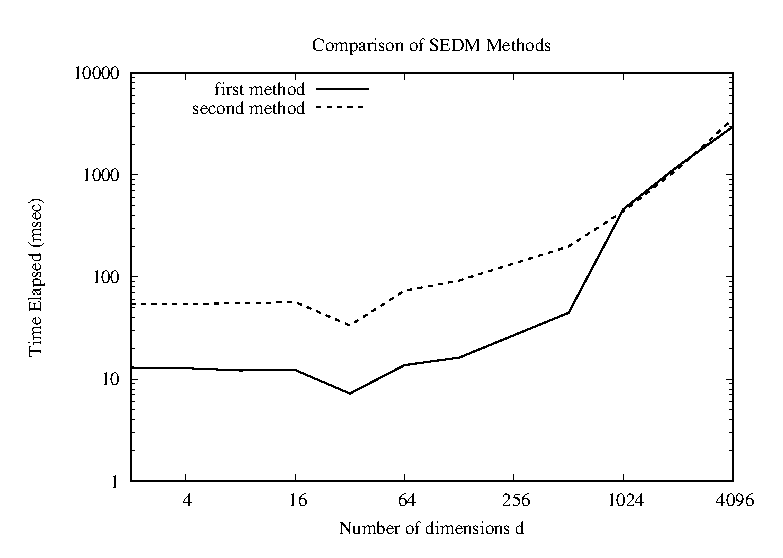
\includegraphics[width=\linewidth]{sedm_d}
	\end{subfigure}%
	\begin{subfigure}{.33\textwidth}
		\centering
		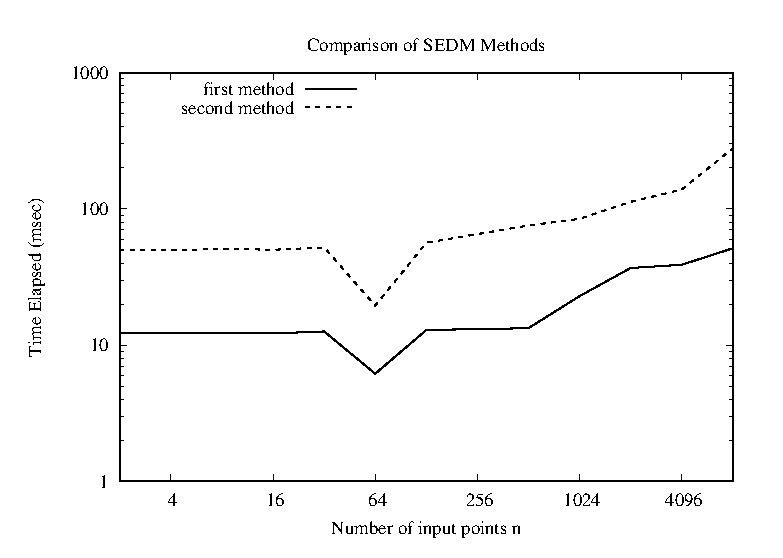
\includegraphics[width=\linewidth]{sedm_n}
	\end{subfigure}%
	\begin{subfigure}{.33\textwidth}
		\centering
		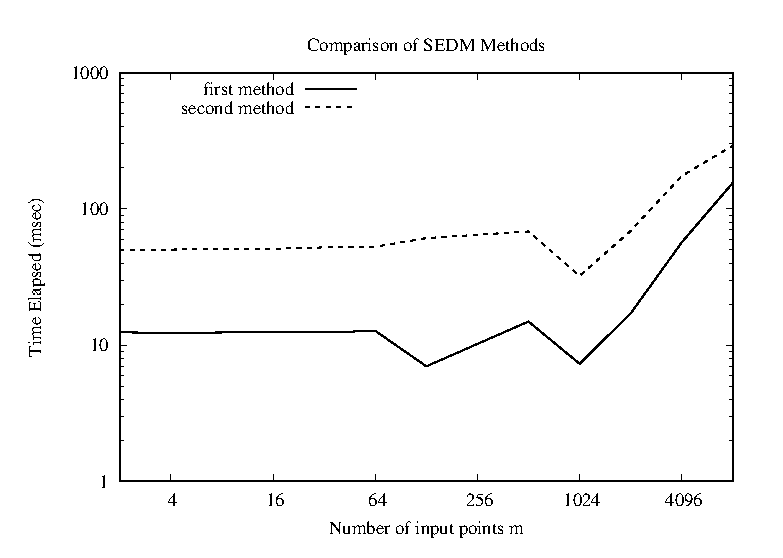
\includegraphics[width=\linewidth]{sedm_m}
	\end{subfigure}
	\caption{Comparison of methods to compute SEDM}
	\label{sedm}
\end{figure}

For the sake of performance, both implementations use \omp \ and \simd \ instructions using \avx \ 
wherever possible, however since shared memory is not the subject of this assignment I will not go into
detail on those.

I decided to use the first implementation for the rest of the program.

\subsection{K-Select}
K-Select refers to a process of selecting the $k$-th smallest element in an array. \\
For this purpose the \qselect \ Algorithm can be used. 

\qselect \ works similar to \qsort, by selecting a random pivot element then seperating the Array into
elements smaller and larger than the pivot. \\
However in \qselect, since we only want the $k$-th smallest
element we check if the new pivot position is larger or smaller than $k$ then we only need to check the 
elements left or right of the pivot. \\
The Algorithm terminates if the pivot position is at position $k$

The array at the end of the algorithm has the $k$-th smallest element at position $k$ and all elements
smaller than it to the left and all elements larger to the right. Since we need the $k$-smallest elements,
we simply read the elements at positions $1$..$k$.

\subsection{KNN}
Finally, to compute the KNN between two arrays of points $X$ and $Y$, meaning for each point $x$ in $X$
find the k-nearest elements $y$ in $Y$, we compute the SEDM $D$ between $X$ and $Y$, then using
\qselect \ for each row in $D$ we obtain the k-nearest neighbours of each element in $X$.

As an additional step, I chose to sort the k first elements of the array before storing using 
\textit{BubbleSort} since it will help in the distributed part of the algorithm.

To compute All-KNN for the array $X$ we simply use the same algorithm with $X$ as both inputs $X$ and $Y$.

Once again, \omp \ is used to improve the performance.

\section{Using MPI}
In order to distribute the problem to $p$ independent nodes we must split our input set into
$p$ sub-sets, where each node takes a sub-set of the input array. It must then compate its own 
sub-set $X$ with itself and all other sub-sets $Y$ in other nodes.

The procedure is the following:
\begin{enumerate}
	\item The root process initializes the various variables by reading the input arguments
		and broadcasts the relevant values to the other processes.
	\item The root process reads the input array from the input device part by part, then sends each
		sub-array to its corresponding node.
	\item Each process initializes $X$ and $Y$ to be the sub-set received.
	\item Each process computes the KNN of $X$ with $Y$, if it has computed the KNN before it
		compares the previous KNN to the new one and merges the 2 results. \label{main_loop}
	\item It send $Y$ to the next process in the ring then recieves into $Z$ the array sent by 
		the previous process.  It then swaps $Y$ and $Z$.
	\item If it has received all parts of the input array then it proceeds to step \ref{printing}. Else it 
		goes back to step \ref{main_loop}.
	\item Then each process sends its KNN result to the root process. The root process receives each result 
		one by one and prints it to the output device. \label{printing}
\end{enumerate}

Care is taken to use non-blocking operations when possible in order to hide the communication costs.

There are 2 parts of this process which require special attention.

\subsection{Merging KNN Results}
Consider the case where a process has computed the KNN for $X$ with the points in $Y_1$.
Then after receiving the next input points it computes KNN for $X$ with $Y_2$.

Each of these contains $k$ points for each point in $X$. We must somehow merge these to obtain
the $k$ smallest elements of both arrays.

The process is similar to the Merging procedure in \textit{MergeSort}.

We create 2 pointers each pointing to the first element in each KNN array. We read the distances at each
pointer then copy the smallest of these to the new KNN array. We then move the pointer to the next element
in the corresponding array. This process is repeated $k$ times until the new KNN array is full.

For this to work the 2 arrays must be sorted, which is why the elements are 
sorted before saving the KNN results.

\subsection{Memory Management}
Let's assume that floating point variables take $F$ bytes of memory and integer type variables $I$ bytes.

$X, Y$ and $Z$ are floating point matrices of size $n \times d$. Collectively they take up 
$3 \cdot n \times d \cdot F$ bytes of data.

The KNN result contains 2 arrays for each point in $X$, one that has the distances to 
each nearest neighbour, and one that holds its index. This means that each KNN result takes up
$n \times k \cdot (I + F)$. 
There may be up to 2 KNN results allocated at each point in time (the previous and the new one) so in total
KNN results take up $2 \cdot n \times k \cdot (I + F)$.

Finally for the KNN computation we must compute the SEDM between $X$ and $Y$. Normally this would be
$n \times n \cdot F$ bytes of memory. However $n \times n$ may be too large to fit in memory. For this 
reason we actually slightly change the way the KNN procedure works.

Instead of computing the entire SEDM once, we split $X$ into slices of length $t$ then compute the KNN
for each slice of $X$ one at a time.
This makes the memory required for the SEDM equal to $n \times t \cdot F$. An additional matrix of the same
dimensions is needed to hold the indices of the elements. These 2 together are $n \times t \cdot (F + I)$
bytes of memory.

In order to determine the size of parameter $t$ we must know the total memory in bytes that is allowed to each
process. I will call this $M$.

Since each of these arrays are of size $n$, we can consider $M$ as a grid with dimensions $n$ and $M/n$

then $X, Y, Z$ take $3d \cdot F$ slices of the grid, KNN results $2k \cdot (F + I)$ slices and
the Distance and Index arrays $t \cdot (F + I)$ slices.

As such, to maximize $t$ we can use the following formula. 
\begin{equation}
	t = \frac{M/n - 3d \cdot F - 2k \cdot(F + I)}{F + I}
\end{equation}

Obviously, there is no reason to use a value of $t$ larger than $n$, so we set it as the minumum of the 2.

\section{Testing and Results}
In this exercise I created various tests in the course of development, in order to check the correctness,
and see the performance of the various methods. 

\subsection{Testing KNN}
To test the correctness of the KNN method, I used a regular grid $G \subset \mathbb{Z}^d$ of points 
in $d$ dimensions. 

For each point $x$ which is not on the edge of the grid, we can test for the correctness of the result by 
evaluating that the nearest neighbours are the points in the ``cage'' $C_x \subseteq G$ around the
specified point, meaning the points $y \in C_x$ such that 
\begin{gather*}
r = x - y = \left[ r_1 \  r_2 \ \ldots \ r_d \right] \\
\forall i \leq d: |r_i| \leq 1
\end{gather*}

And since $x, y \in G \subseteq \mathbb{Z}^d$ it is true that 
$\forall x \in G ,y \in C_x, i: r_i \in \{-1, 0, 1\}$.

Obviously, there are $3^d$ such points since we are examining a $3 \times 3 \times \ldots \times 3$ cage,
but also from a combinatronics point-of-view, $r$ has $d$ dimensions, each having $3$ possible values, so 
in total $3^d$ combinations of points. 

The combinatronics perspective can also be used to determine how many points in $C_x$ are at a specified
distance from $x$. Specifically, to get the number of points in $C_x$ which are at distance $s$ from $x$, 
meaning the number of points $r = x - y$ where $||r||^2 = s$ \footnote{Since we are using the Squared Euclidean 
Distance}. 

Then, since $\forall i: |r_i| \in {0, 1}$ then $||r||^2 = |r_1|^2 + |r_2|^2 + \ldots + |r_d|^2 = 
|r_1| + |r_2| + \ldots + |r_d| = s$ means that there must be $s$ elements $r_i$ where $|r_i| = 1$ 
and $d - s$ elements where $|r_i| = 0$. There are $d \choose s$ such combinations.

For each of these combinations, there are $s$ elements where $|r_i| = 1$, meaning $r_i \in {-1, 1}$.
As such, for each of the $s$ elements there are $2$ possible values, meaning there are $2^s$ such 
combinations.

In total, the formula to get the number of combinations such that $||r||^2 = s$ is
\begin{equation}
	\#\{ r^2 = s \} = {d \choose s} \cdot 2^s \hspace{12pt} 0 \leq s \leq d
\end{equation}

From this we can conclude that \\
there is $1$ combination for $s = 0$, which makes sense as each point is unique\\
$2d$ combinations for $s = 1$, corresponding to 2 points along each dimension \\
and $2^d$ combinations for $s = d$, which correspond to the number of corners of a $d$-dimensional hypercube.

These results can be compared against the output of the program in order to check their correctness.

\subsection{Testing Performance}

Figure \ref{knn}. shows the relationship between various input parameters and the performance of the algorithm
\footnote{Most of the graphs are in log-log scale, using arbitrary values for the fixed parameters}.

The size $n$ of the input array seems to be constant up to a specific size then have 
$\mathrm{O}(n^2)$ complexity afterwards. 
As for $k$ it seems to not affect the performance significantly in the range I tested, 
but it seems that it may increase with $\mathrm{O}(k^2)$ for larger values of $k$
\footnote {This is probably due to \textit{BubbleSort} and could be improved}.
The number of processes seems to be inversly proportional to the required time, 
while the Memory per Process used improves performance up to a certain point, 
after which the entire SEDM fits in memory and it no longer has any effect.

\begin{figure}[h]
	\centering

	\begin{subfigure}{.4\textwidth}
		\centering
		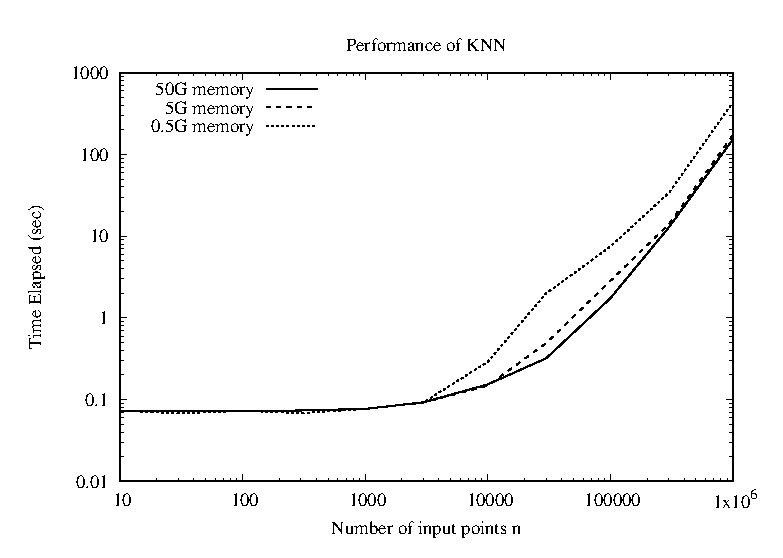
\includegraphics[width=\linewidth]{knn_n}
	\end{subfigure}%
	\begin{subfigure}{.4\textwidth}
		\centering
		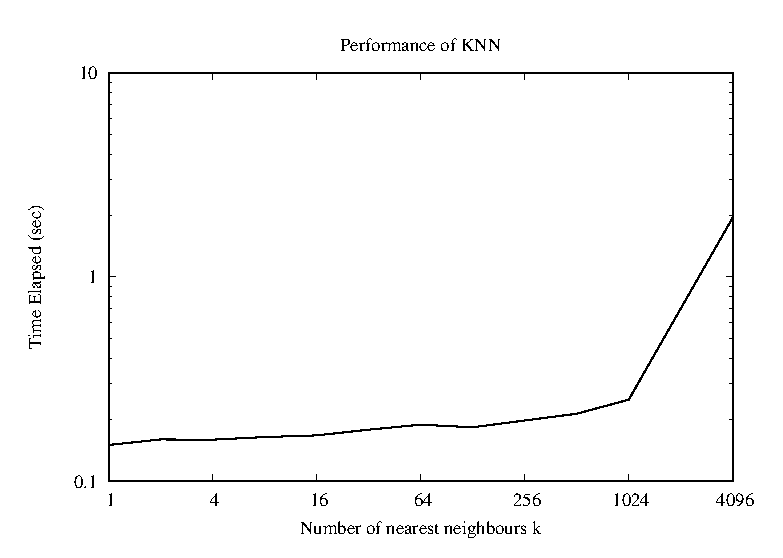
\includegraphics[width=\linewidth]{knn_k}
	\end{subfigure}

	\begin{subfigure}{.4\textwidth}
		\centering
		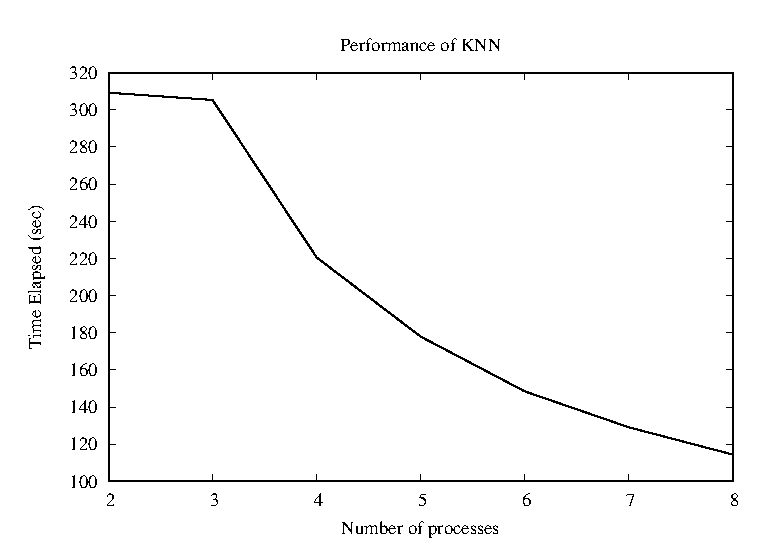
\includegraphics[width=\linewidth]{knn_p}
	\end{subfigure}%
	\begin{subfigure}{.4\textwidth}
		\centering
		\includegraphics[width=\linewidth]{knn_mem}
	\end{subfigure}

	\caption{The performance of the KNN method using MPI related to various parameters}
	\label{knn}
\end{figure}

\subsection{Working with the `AUTH IT Compute Cluster' and SLURM}
Most of the results shown were obtained using the computing power of the `Aristotelis' HPC. To this end, 
I had to work with the \slurm \ Workload Manager. The computing resources offered were not only 
absolutely necessary in order to compute the KNN Results for very large inputs, but also very impressive.
However, \slurm \ itself turned out to be a bit of a pain. 

Firstly, the documentation --though it exists-- is pretty lacking in terms of detailed
explanations of the various parameters. In general I found BATCH scripts somewhat limiting.

Secondly, the queue times are quite long. Most of the time the majority of computer nodes will be taken up by
processes which have allocated 1 to 2 days of compute time, and do in fact take near 2 days to complete. 
This makes it difficult to find the available resources especially for high node counts.
For this reason many of the results were obtained using just 2 or 3 nodes, the processes split between them
when necessary.

\subsection{Notes and Feedback}
Since this is the $5^{th}$ page of the report \footnote{``Sin first, Then ask for forgiveness'' was mentioned},
and may be ignored anyway, I will take the chance to be a little less formal in this section.

I want to mention a few things I found interesting, what I have learned, and a few ways I messed up.

I'll be the first to admit that I did not manage my time correctly at all this time
(even taking into account that it was the holidays).
I started working on implementing the SEDM methods early on but the rest of the
project was completed in the last ten days or so.

This initially caused somewhat of a panic (since the deadline was originally much earlier),
so while not cutting corners per se, I did not exactly polish them clean either. 
This shows itself in multiple parts of the code: \\
almost no error checking \footnote{This has in the past been referred to as ``bravery''}, 
lacking code documentation and probably a few instances of spaghetti code. 

The entire codebase could use refactoring
(for example the `knn' function comically having 9 input parameters).

The other effect this had was that I did not have time to implement some things I wanted to do.\\
Some of these (probably in order of importance) are:
\begin{enumerate}
	\item Script to validate the correctness of the KNN results on Regular Grids (I had to do this manually)
	\item Script to generate arbitrary size input arrays (I can only generate hyper-cubic regular grids)
	\item Better memory management
	\item Testing on classification datasets like MNIST
	\item More testing in general
	\item Try using other \blas \ libraries
	\item Consider more k-selection algorithms
	\item Implement other distance metrics
	\item Shorten this report to be contained within 4 pages 
\end{enumerate}

Nonetheless, I enjoyed this assignment, probably more than the first one. Mathematics take up
a significant part of the report which might be considered unnecessary, but for me it was
one of the most interesting parts of assignment and I did not want to exclude them (I would have probably
written more if I had the space).

Working with \mpi \ is definitely more difficult than working with \omp, but it was quite interesting.
Having to think about the project at both the process level and the communication level was a good challenge.

Working with the HPC cluster was also very interesting.
Being able to work with that much computing power is very impressive
\footnote{I am writing this using a 4 core i5 and do not own a gaming PC}, 
though my grievances with \slurm \ have been made clear.

So finally, what I learned from this is to try and manage my time better (I will try to do
so in the next assignment) and to start testing early so I can have results despite the long queue.
Using helper scripts and automated testing really helped this time so I will also try to use more of these
in the future.

\end{document}
